\documentclass[11pt]{article}

\usepackage{url}
\usepackage[letterpaper,margin=1in]{geometry}
\usepackage{times}
\usepackage{graphicx}


\begin{document}

\title{SqueezeDB: \\ Approximate Queries on Large Scientific Data}
\author{Justin A. DeBrabant \\ debrabant@cs.brown.edu \and Gideon
  Goldin \\ gideon\_goldin@brown.edu \and Duy Nguyen \\ duy@cs.brown.edu}
\date{Final Project - CSCI 2950t - Fall 2011}
\maketitle

\begin{abstract}
In this paper, we present a system for computing approximate queries
on large scientific data with confidence bounds using the VC-Dimension
estimation of query selectivity. We provide an overview of the system
as well as the experimental results that show the accuracy and
performance of our estimation techniques. 
\end{abstract}

\section{Introduction}
\label{sec:intro}
We are in the midst of a data revolution. As data collecting
technologies have increased in both quality and scope, the amount of
data that is being acquired on a daily basis has exploded. In many
cases, existing data management and data analysis tools have struggled
to keep up. Nowhere is this trend more apparent than in the scientific
community where the data is often being generated on the scale of
terabytes daily. A prime example of this is the Sloan Digital Sky
Survey (SDSS) whose goal was a complete 3-dimensional mapping of the
night sky using a 125-megapixel camera. To date, the SDSS has produced
almost 100 TB of filtered and tagged data. This was a massive
international accomplishment and scientists are only beginning to
explore the data available. 

The obvious question when dealing with data at this scale is how does
one even go about exploring it. Clearly, downloading the data to a
local hard drive and issuing queries or running scripts to extract
information is infeasible, as scanning that magnitude of data could
take weeks. Also, because the questions being asked are often
exploratory, the cycle would be iterative. In this paper, we present
SqueezeDB, a system for running approximate queries on sampled data
and bounding the confidence of the results. Using the VC-dimension to
estimate query result selectivities, we are able to execute aggregate
queries on a subsample of the whole data and get very accurate
results. The aggregate queries on the sampled data are often orders of
magnitude faster than the same queries on the entire dataset and thus
give the researcher the opportunity to explore and analyze the data in
a reasonable amount of time.

\section{Background and Related Work}

This is not the first work on sampling large data and running
approximate queries on the sample. In \cite{Hellerstein}, Hellerstein
et al. presented the idea of online query results with confidence
bounds. They used Hoeffding inequalities to show the progress of a
given query, the result so far and finally a confidence that the shown
result was within the confidence interval. This was one of the first
works in providing approximate results for long-running queries. As a
follow up on \cite{Hellerstein}, Haas et al. presented a method for
bounding confidence of results on a sample of the actual dataset in
\cite{Haas}. While the end goal of this is the same as our project,
there are a few key differences. The most obvious is how the sample of
the data is acquired. In \cite{Haas}, they must sample the data
``online'', after a query is sent to the system. Thus, for each query,
a new sample must be constructed. While in most cases this will still
be significantly faster than querying the full dataset, there is still
significant overhead involved in the sampling. In our approach, the
sample is created once, offline, and can be used for all the queries
in the specified query workload. Their approach also differs from our
in how the confidence bounds are computed. They use Hoeffding
inequalities while we use the VC-Dimension to estimate query
selectivity presented in \cite{Matteo}. These different theoretical
frameworks provide different approximate answers and confidence
bounds. In \cite{Aqua}, the authors present AQUA, a complete system
for approximate query processing. Aqua acheives approximate query
answers by maintaining a large amount of synopses (i.e. summary
information) about the tables in the database. There are also no
confidence bounds in this approach.

\section{SqueezeDB}

\subsection{System Overview}

SqueezeDB, our implementation of approximate query processing and confidence
bounds calculation, is based on the VC-DImension method for query
selectiviy estimation. We omit the theoretical details in this paper
and instead refer the reader to \cite{Matteo}. Instead, we focus on
the system architecture necessary to make the approximate query
possible. We have implemented SqueezeDB as a wrapper on top of
PostgreSQL. We provide a front-end GUI where the user enters parameter
values into a query template. In order to compute the confidence
bounds, we must solve an optimization problem. Depending on the
aggregate function being computed (i.e. SUM, AVG, COUNT, $\ldots$),
the optimization problem will can either be linear or non-linear, but
in all cases will be convex, and thus solveable. Our experimental
evaluation has shown that they type of optimization problems we are
solving are simple in practice and the use of external optimization
libraries can be done in real-time and sitll provide significant
performance improvements over querying the non-sampled dataset. For
linear optimization problems (only SUM), we use the CPLEX optimization
library. For non-linear optimization problems use use Python's APM
package. 

\subsection{System Implementation}

There are two distinct phases in our system:  an offline and an online
phase. The offline phase is used to create the sample and all
necessary data statistics. During the online phase, we use query
rewriting to redirect the approximate query to the sampled database
and then solve the corresponding optimization problem based on the
query result. The details of these phases are given below.

\subsubsection{Offline Phase}

Because our sample is used for every query in the query workload, we
can create and store the sample offline. According to \cite{Matteo},
the size of the sample needed is independent of the size of the
original dataset, and instead only depends on the complexity of the
queries in the query workload. The complexity of the queries is a
function of the maximum number of joins, columns and boolean clauses
that will be present in all the queries that the system will
process. Our theoretical guarantees for confidence bounds are valid as
long as no query received is above the maximum numbers given during
this offline phase. Given these maximums, we determine the appropriate
sample size, create the sample from the dataset using uniform random
sampling and store the newly constructed sample in a table alongside
the original dataset. Note, for simplicity we are assuming that the
original dataset is stored as one large table and as such the sample
can be stored in a single table as well. This is not a necessary
assumption and was made simply for ease of presentation. If multiple
tables are present in the original data, a sample size and the
corresponding sample will be created for each table
independently. Thus, for a dataset with $n$ table, the resulting
database will contain $2n$ total tables, $n$ original tables and $n$
sample tables. Also in the offline phase, we construct a catalog of
statistics about the data.  These statistics include the number and
name of the columns in the database (used by the GUI), the maximum and
minimum value for each column in the database (needed for the
confidence interval optimization problem) and the original data and
sample size (in terms of rows).

\subsubsection{Online Phase}

In the GUI, the user is given the ability to construct the query from
a given template and the given the option to compute the exact or the
approximate result. In the case that the exact result is desired, the
procedure is simple, we submit the query unchanged to the
underlying PostgreSQL database and return the results to the user. For
the approximate case there is much more to do. The query is first
passed to the Query Parser. The job of the Query Parser is to rewrite
the query to use the sampled table as well as determine the max/min
values for each column in the query, which are needed for the
optimization problem. The Query Parser is also responsible for
replacing the aggregate function in the SELECT clause to be a SELECT
(*). This is done because for our approximation, we need the actual
rows to be returned, not the result of the aggregate computation. We
will compute the aggregate result client-side. For example, consider the simple query below: 

\begin{center}
SELECT SUM(c\_1) FROM table1 WHERE c\_1 $<$ 10; 
\end{center}

\noindent If an approximate result is desired, the Query Parser will
rewrite the query to the following: 

\begin{center}
SELECT * FROM table1\_sample WHERE c\_1 $<$ 10; 
\end{center}

\noindent where table1\_sample is the sampled version of table1 (we get
this information from the system catalog, which is queried at system
startup). In this case, the column max for c\_1 is 10 and the minimum
is whatever the absolute minimum for column c\_1 is, which would also
be stored in the system catalog. The max/min for all the other columns
would be the absoluted min/max values stored in the system
catalog. After the query is rewritten, it is submitted to the postgres
database. The results returned will be a set of rows that meet the
query predicates. The system must now compute the confidence bounds as
well as the aggregate function result, which will both be returned to
the user. An overview of this process can be seen in Figure
\ref{fig:overview}. 

\begin{figure}
\centering
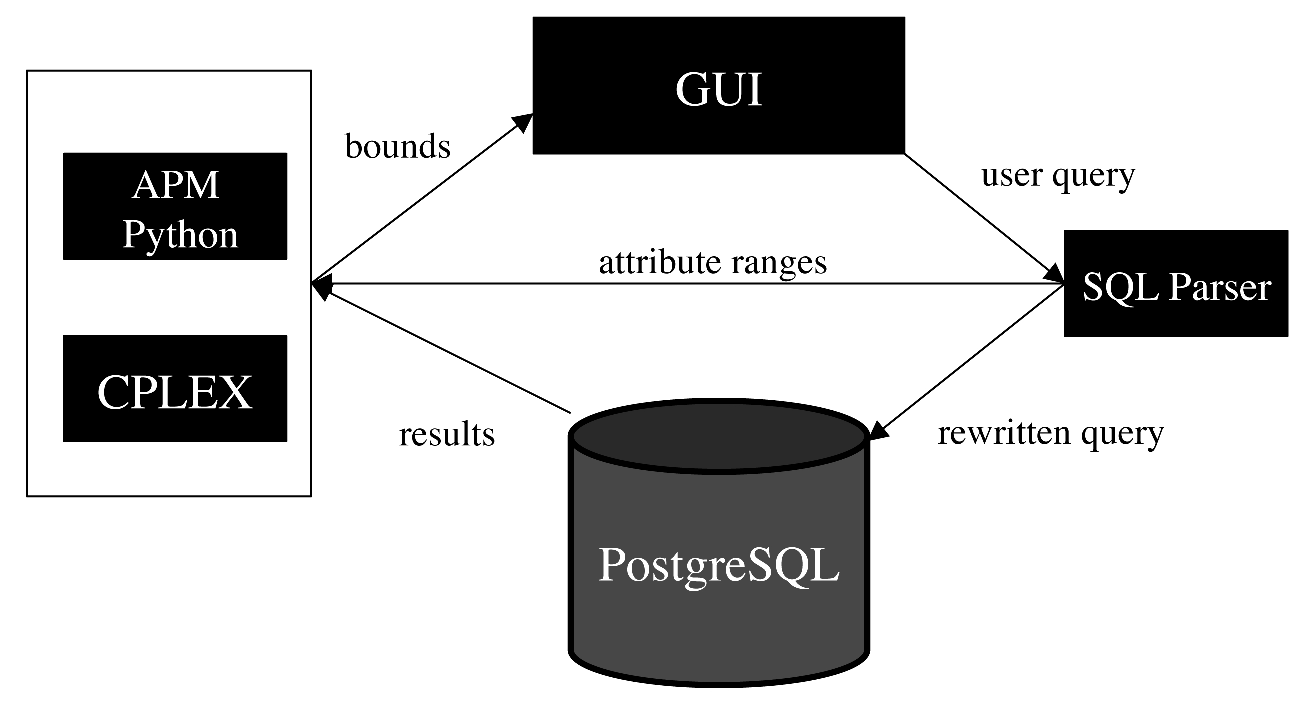
\includegraphics[width=0.7\textwidth]{overview}
\caption{An overview of approximate query processing in SqueezeDB.}
\label{fig:overview}
\end{figure}

\section{Experimental Evaluation}

In our experimental evaluation, we wanted to test both the correctness
and performance of our approximate query processing approach. Clearly,
if solving the optimization problem to calculate the confidence bounds
takes longer than executing the query on the full dataset then there
is no benefit to our approach. To test this, we used a 75GB sample
dataset with 1 billion tuples. Each tuple contained 10 integer
columns. The value for each column was randomly generated from a range
of [0, 100000]. The query workload we ran was also randomly generated
by selecting up to 3 columns and 5 boolean clauses in the WHERE clause
for each query. Based on this query complexity (0 joins, 3 columns,
and 5 boolean clauses), we computed (using the formula in
\cite{Matteo}) that we would need approximately 19000 rows in our
sample, which were sampled randomly with replacement. Notice the
\emph{significant} data reduction in this example (from 1000000000 to 19000
rows). While our experiments were admittedly simple, it does
demonstrate the massive data reduction that is possible using
approximate queries on sampled data. We ran 5 of the queries from our
benchmark with the results shown in Figure \ref{fig:results}. The
immediate takeaway from our experimental evaluation was that although
the approximation value was very accurate (never more than 2\% from
the actual value), the confidence bounds were extremely
loose. However, considering that we were running queries on 19000 rows
instead of 1 billion and getting results within a few percent, we
believe there is still value in this approximation method.

\begin{figure}
\centering
\begin{tabular} {| l | l | l | l | l |}
\hline
& relative sum accuracy & runtime improvment & min bound & max bound \\
\hline
Q1 & .3\% & 99.999\% & 71\% & 78\% \\
\hline
Q2 & .6\% &  99.999\% & 99\% & 30\% \\
\hline
Q3 & 1.3\% &  99.999\% & 60\% & 46\% \\
\hline
Q4 & 1.6\% &  99.999\% & 33\% & 79\% \\
\hline
Q5 & 1.7\% &  99.999\% & 68\% & 90\% \\
\hline
\end{tabular}
\caption{Eperimental evaluation of the methods implemented in
  SqueezeDB. The relative sum accuracy is how close the approximate
  aggregate was to the exact aggregate. The runtime improvement is the
decrease in runtime for the approximate query compared to the exact
query. The min and max bound are the confidence intervals of the
approximate query with respect to the original aggregate result. For
example, a result of 100 with a min/max bound of 50\% would mean a
confidence interval of [50, 150].}
\label{fig:results}
\end{figure}

\section{Conclusions}

In this paper we presented a system for approximating queries run on
sampled data. We implemented a prototype system named SqueezeDB that
acted as a wrapper around PostgreSQL and allowed the user to either
execute exact or approximate queries. Using query rewriting and
several external tools (CPLEX, APM Python), we were able to make the
process of approximate query processing transparent to the user. 

We also prsented an experimental evaluation of our methods and
concluded that while the approximation itself, in practice, was very
accurate, the theoretical guaranteed confidence bounds were far too
loose. For future work, we intend to continue to develop the theory
behind the confidence bounds in an effort to make them tighter. We
also plan to continue developing SqueezeDB by adding more support for
approximate queries such as variance or median. 


\bibliographystyle{plain}
\bibliography{report}

\end{document}
